\chapter{Theoretische Grundlagen}

\section{Begriffsdefinitionen}
In den folgenden Kapiteln werden die Begriffe ``Social Network Analysis'', ``Social Forces'', ``Graph'' und ``Link-Prediction'' einzeln
erläutert. Es handelt sich in Bezug auf die Arbeit um grundlegende Begriffe. Weitere Fachbegriffe, die
in der Arbeit verwendet werden, sind im Glossar beschrieben.
% TODO Make glossary

\subsection{Social Network Analysis}
Soziale Netzwerke bestehen aus Akteuren, wie beispielsweise Individuen, Organisationen oder ganze Nationen und deren Beziehungen (\citeauthor{ulrike_baumol_soziale_2019} \citeyear{ulrike_baumol_soziale_2019}, online).
Unter \acl{sna} (SNA, dt. Soziale Netzwerkanalyse) wird die Methode zur Erfassung und Analyse von dieser Netzwerke und der Beziehungen darin verstanden (\citeauthor{wikipedia_soziale_2019} \citeyear{wikipedia_soziale_2019}, online).
Die soziale Netzwerkanalyse ist ein interdisziplinäres Forschungsfeld und wird nach \cite{ulrike_baumol_soziale_2019} in den Sozial- und Verhaltenswissenschaften aber auch in der Betriebswirtschaftslehre oder den Politikwissenschafften angewandt.
Gegenwärtig sind sogenannte "soziale Netzwerke" allgegenwärtig und werden insbesondere im Kontext von Internet-Plattformen wie \textit{Facebook} oder \textit{Twitter} häufig betrachtet.

\subsection{Social Forces}
\label{socialforces}
%TODO Write section

\subsection{Graph}
Soziale Netzwerke können einfach als Graph modelliert werden.
Ein Graph $G = (V, E)$ besteht aus einer Menge $V = \{1,2,...,|V|\}$ von Knoten und Kanten $E \subseteq V\times V $ (vgl. \citeauthor{ottmann_algorithmen_2017}, \citeyear{ottmann_algorithmen_2017}, 154). % TODO Verify pagenumber
Die Knoten repräsentieren dabei Akteure, während die Kanten die Beziehungen zwischen den Akteuren repräsentieren.
Abbildung \ref{fig:graph_undirected} zeigt einen ungerichteten Graphen. Die Kanten enthalten dabei keine Pfeile, was verdeutlicht, dass die Interaktion in beide Richtungen erfolgen kann.
Ein Beispiel für einen ungerichteten Graphen ist das Freundes-Netzwerk von \textit{Facebook}.

\begin{figure}[h]
    \centering
    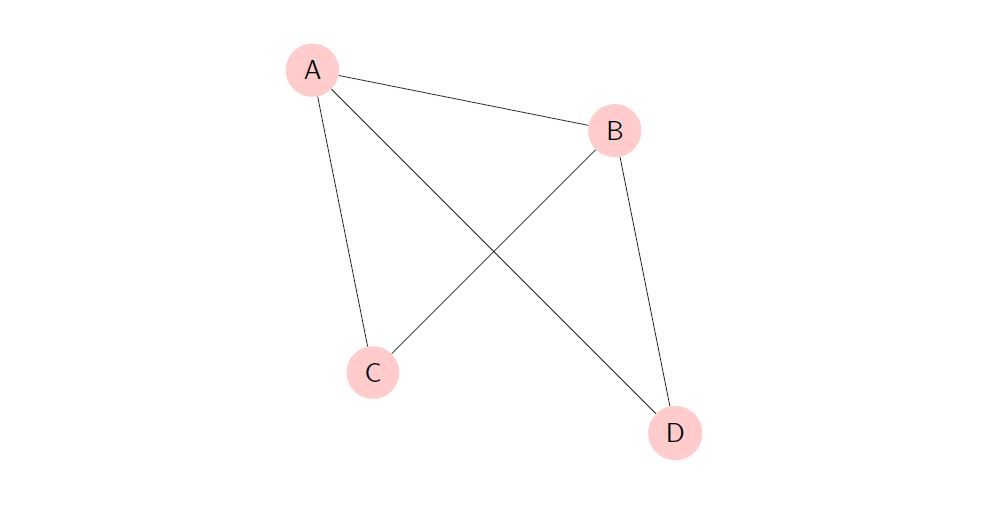
\includegraphics[scale=0.7]{resources/graph_undirected.JPG}
    \caption{Ungerichteter Graph}
    % TODO Add cite to SNA Script
    \label{fig:graph_undirected}
\end{figure}

Im Gegensatz dazu gibt es bei einem gerichteten Graphen eine Quelle und ein Ziel. Die Richtung der Interaktion wird durch einen Pfeil visualisiert.
Abbildung \ref{fig:graph_directed} zeigt einen solchen Graphen.
Als Beispiel für einen gerichteten Graphen dient ein E-Mail Netzwerk. Jede Nachricht wird dabei von einem Sender an einen Empfänger versendet.

\begin{figure}[h]
    \centering
    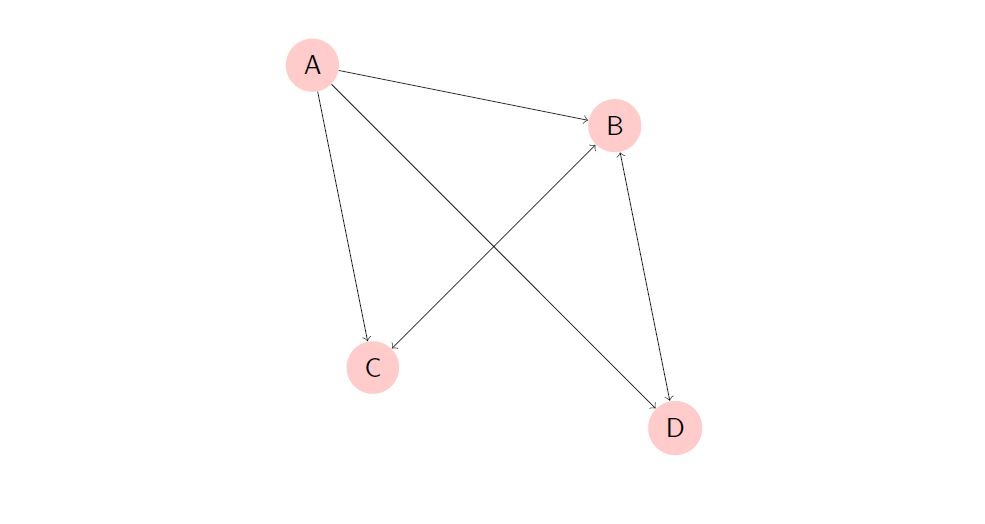
\includegraphics[scale=0.7]{resources/graph_directed.JPG}
    \caption{Gerichteter Graph}
    % TODO Add cite to SNA Script
    \label{fig:graph_directed}
\end{figure}

\subsection{Link-Prediction}
Link-Prediction baut auf einem bestehenden Netzwerk auf und versucht vorherzusagen, welche Kante sich als nächstes Bilden werden:
Der Graph $G = (V, E)$, bestehend aus Knoten ($V$, en.: Vertices) und Kanten ($E$, en.: Edges), hat sich in einem Zeitintervall $G[t, t1]$ gebildet.
In einem nächsten Zeitintervall $G[t1, t2]$ könnten neue Kanten zum Netzwerk hinzukommen.
Mittels Link-Prediction wird nun versucht vorherzusagen, welche Kanten in welcher Reihenfolge zum Graphen hinzugefügt werden (\cite{gao_link_2015}, 4).
Für solche Vorhersagen gibt es verschiedene Algorithmen mit unterschiedlichen Charakteristiken.
Je nach Eigenschaften des vorliegenden Netzwerks und allfälliger Kontextinformationen liefert ein Algorithmus bessere oder schlechtere Resultate.
Pro Anwendungsfall muss deshalb evaluiert werden, welcher Algorithmus sich am besten eignet.
Der Aufbau der dazu benötigten Messwerte und die darausfolgende Evaluation wird im Kapitel \ref{daten} beschrieben.
